Learning from interactions with users is ubiquitous in modern customer-facing systems, from product recommendations to web search to spam detection to content selection to fine-tuning the interface. Many systems purposefully implement \emph{exploration}: making potentially suboptimal choices for the sake of acquiring new information. Randomized controlled trials, a.k.a. A/B testing, are an industry standard, with a number of companies such as \emph{Optimizely} offering tools and platforms to facilitate them. Many companies use more sophisticated exploration methodologies based on \emph{multi-armed bandits}, a well-known theoretical framework for exploration and making decisions under uncertainty.

%~\cite{KohaviAB-2015,KohaviLSH09}

Systems that engage in exploration typically need to compete against one another; most importantly, they compete for users. This creates an interesting tension between \exploration and \competition. In a nutshell, while exploring may be essential for improving the service tomorrow, it may degrade quality and make users leave \emph{today}, in which case there will be no users to learn from! Thus, users play three distinct roles: they are customers that generate revenue, they generate data for the systems to learn from, and they are self-interested agents which choose among the competing systems.

We initiate a study of the interplay between \exploration and \competition. The main high-level question is: {\bf whether and to what extent competition incentivizes adoption of better exploration algorithms}. \gaedit{This translates into a number of more concrete questions. While it is commonly assumed that better learning technology always helps, is this so for our setting? Does increasing competition lead to higher consumer welfare? To what extent does one firm possessing more information or having a better perception amongst consumers than its competitors serve as a barrier to entry in this environment?

We investigate these questions for two separate but connected models. In the first we suppose that consumers are well-informed about the firm's exploration strategies but do not observe any information about past user experiences with the firms. In the second, we suppose that consumers \textit{only} consider the average of past user experiences with each of the firms. In the first model we analytically characterize the equilibrium exploration strategies of two firms competing for the same stream of consumers as we vary the degree of randomness in consumer decisions.\footnote{The randomness in consumer decisions can be interpreted both as the degree of rationality as well as a reduced-form way of capturing the degree to which consumers themselves engage in exploration} In the second model we account for competition in a more direct way and utilize numerical simulations to consider asymmetries in the timing of entry, increasing competition beyond two firms, and allow us to isolate the effect that role that data can play as a barrier to entry.

On a high level, our contributions can be framed in terms of the ``inverted-U relationship" between competition and the quality of adopted algorithms (see \reffig{fig:inverted-U}).

}

\begin{figure}
\begin{center}
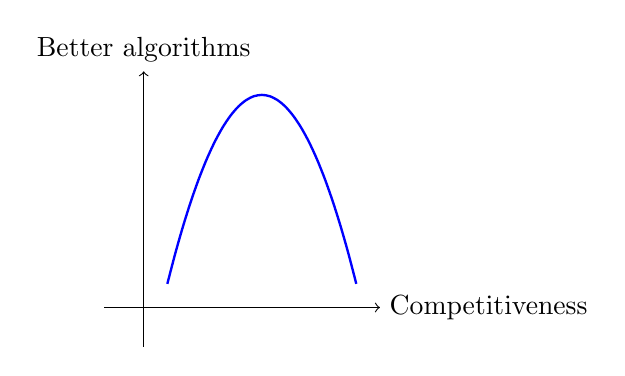
\begin{tikzpicture}
      \draw[->] (-.5,0) -- (3,0) node[right] {Competitiveness};
      \draw[->] (0,-.5) -- (0,3) node[above] {Better algorithms};
      \draw[scale=0.6,domain=0.5:4.5,smooth,variable=\x,blue, line width=0.3mm] plot ({\x},{4.5 - (\x - 2.5)^2});
      % \draw[scale=0.5,domain=-3:3,smooth,variable=\y,red]  plot ({\y*\y},{\y});
 \end{tikzpicture}

\caption{Inverted-U relationship between rationality/competitiveness and algorithms.}
\label{fig:inverted-U}
\end{center}
\end{figure}



% the extent to which the game between the two principals is competitive
% degree of innovation that these models incentivize.
% the extent to which agents make rational decisions


%\subsection{Our model}
%\label{sec:intro-model}

\xhdr{Our model.} We define a game in which two firms (\emph{principals}) simultaneously engage in exploration and compete for users (\emph{agents}). These two processes are interlinked, as exploration decisions are experienced by users and informed by their feedback. We need to specify several conceptual pieces: how the principals and agents interact, what is the machine learning problem faced by each principal, and what is the information structure. Each piece can get rather complicated in isolation, let alone jointly, so we strive for simplicity. Thus, the basic model is as follows:

\begin{itemize}

\item A new agent arrives in each round $t=1,2, \ldots$, and chooses among the two principals. The principal chooses an action (\eg a list of web search results to show to the agent), the user experiences this action, and reports a reward. All agents have the same ``decision rule" for choosing among the principals given the available information.

\item Each principal faces a very basic and well-studied version of the multi-armed bandit problem: for each arriving agent, it chooses from a fixed set of actions  (a.k.a. \emph{arms}) and receives a reward drawn independently from a fixed distribution specific to this action.

\item Principals simultaneously announce their learning algorithms before round $1$, and cannot change them afterwards. There is a common Bayesian prior on the rewards (but the realized reward distributions are not observed by the principals or the agents).  Each principal only observes agents that chose him. \gaedit{The information set for the agent differs between the two variants of the model. \begin{enumerate}
\item In the first, agents do not receive any other information and choose between the principals using their knowledge of $t$ and the principals' algorithms
\item In the second, agents have access to a reputation score for each principal, which is a sliding window average of the rewards experienced by previous agents that have visited this principal
\end{enumerate}
}
\end{itemize}

\gaedit{
\xhdr{Main Findings.}
In both variants of our model, we find that in a simultaneous entry duopoly a greedy algorithm that does no purposeful exploration is incentivized in equilibrium. In the first variant of the model, once a firm does any exploration it is immediately starved of consumers when its opponent plays a greedy algorithm since we show that the expected reward for every subsequent consumer is higher for the firm that plays the greedy algorithm. In the second variant of the model, the same mechanism drives the greedy algorithm to be incentivized in equilibrium. In this variant, exploration hurts a firm's reputation and decrease its market share in the near term. This leaves the firm with less users to learn from, which may further degrade the firm's performance relative to competitors who keep learning and improving from \emph{their} customers, and so forth. Taken to the extreme, such dynamics lead to a ``death spiral" effect when the vast majority of customers eventually switch to competitors. In both cases, consumer welfare is low since the greedy algorithm is known to be dramatically bad in many important cases of multi-armed bandits.

The primary mechanism that generates this stark result is the same in both variants of the model: consumers need to be incentivized to select a firm over its competitors, leading firms that engage in exploration to be starved of consumers before they make enough progress on their learning problem. In order to incentivize ``better" exploration strategies the key intuition is that the firm needs to have some ``free" consumers to visit them without having to incentivize them. This allows the firm to eventually get out of the hole of exploration.

In the first variant of the model, we relax the decision rule of the consumers to allow for each firm to be chosen with some fixed baseline probability so that firms get a constant stream of ``free" consumers. This can be interpreted as a reduced-form relaxation of the assumption that consumers are myopic and themselves may be engaging in exploration or, alternatively, as deviations from rational behavior. We find that, in this setting, better algorithms help in a big way: a sufficiently better algorithm is guaranteed to win all non-random agents after an initial learning phase. While the precise notion of ``sufficiently better algorithm" is rather subtle, we note that commonly known ``smart" bandit algorithms typically defeat the commonly known ``naive" ones, and the latter typically defeat the greedy algorithm. However, there is a substantial caveat: one can defeat any algorithm by interleaving it with the greedy algorithm. This has two undesirable corollaries: a better algorithm may sometimes lose, and a pure Nash equilibrium typically does not exist.

In the second variant of the model, we keep the decision rule of the consumers but instead vary the timing of entry and allow one firm to have a first-mover advantage so that this firm (denoted as the incumbent) gets all the agents in the market before the other firm enters. We find that, if the first-mover period is sufficiently large, then the incumbent has a dominant strategy to play ``smart" bandit algorithms and that consumer welfare is substantially higher than in the case of simultaneous entry. The intuition is simply that a sufficiently long incumbency period allows the firm to make sufficient progress on its learning problem that it can overcome the original drop in its reputation from exploration in the beginning rounds.

\xhdr{Additional Findings} In the first variant of the model, we further relax the decision rule of the agents so that the probability of choosing a given principal varies smoothly as a function of the difference between  principals' expected rewards; we call it \SoftMaxRandom. For this model, the ``better algorithm wins" result holds under much weaker assumptions on what constitutes a better algorithm. This is the most technical result of the paper. The competition in this setting is necessarily much more relaxed: typically, both principals attract approximately half of the agents as time goes by (but a better algorithm may attract slightly more).

In the second variant of the model, we investigate the ``first-mover advantage" phenomenon in more detail. Being first in the market gives free data to learn from (a ``data advantage") as well as a more definite, and possibly better reputation compared to an entrant (a ``reputation advantage"). We run additional experiments so as to isolate and compare these two effects. We find that either effect alone leads to a significant advantage under competition. The data advantage is larger than reputation advantage when the incumbent commits to a more advanced bandit algorithm.

Data advantage is significant from an anti-trust perspective, as a possible barrier to entry. We find that even a small amount ``data advantage" gets amplified under competition, causing a large difference in eventual market shares. This observation runs contrary to prior work  \cite{lambrecht2015can,bajari2018impact}, which studied learning without competition, and found that small amounts of additional data do not provide significant improvement in eventual outcomes. We conclude that competition dynamics -- that firms compete as they learn over time -- are pertinent to these anti-trust considerations.

We also investigate how algorithms' performance ``in isolation" (without competition) is predictive of the outcomes under competition. We find that mean reputation -- arguably, the most natural performance measure ``in isolation" -- is sometimes not a good predictor. We suggest a
more refined performance measure, and use it to explain some of the competition outcomes.

\OMIT{All results extend to a much more general version of the multi-armed bandit problem in which the principal may observe additional feedback before and/or after each decision, as long as the feedback distribution does not change over time. In most results, principal's utility may depend on both the market share and agents' rewards.
}
\xhdr{Economic interpretation.}
The inverted-U relationship between the severity of competition among firms and the quality of technologies that they adopt is a familiar theme in the economics literature \citep[\eg][]{Aghion-QJE05,Vives-08}.%
\footnote{The literature frames this relationship as one between ``competition" and ``innovation". In this context, ``innovation" refers to adoption of a better technology, at a substantial R\&D expense to a given firm. It is not salient whether similar ideas and/or technologies already exist outside the firm. It is worth noting that the adoption of exploration algorithms tends to require substantial R\&D effort in practice, even if the algorithms themselves are well-known in the research literature; see \citet{MWT-WhitePaper-2016} for an example of such R\&D effort.}
We find it illuminating to frame our contributions in a similar manner, as illustrated in \reffig{fig:inverted-U}.

In our model, competition varies based on the number of ``free" consumers that a firm receives. In the first variant of the model, this comes from introducing ``random" consumers where we vary from fully rational decisions with \HardMax to relaxed rationality with \HardMaxRandom to an even more relaxed rationality with \SoftMaxRandom. Indeed, with \HardMax you lose all customers as soon as you fall behind in performance, with \HardMaxRandom you get some small market share no matter what, and with \SoftMaxRandom you are further guaranteed a market share close to $\tfrac12$ as long as your performance is not much worse than the competition. The uniform choice among principals corresponds to no rationality and no competition. In the second variant of the model, this comes from the number of firms and the timing of entry in the market. Competition in this case ranges from monopoly to ``incumbent" (first-mover in duopoly) to simultaneous entry duopoly to ``late entrant" (last mover in duopoly). The same distinctions in both cases also control the severity of competition between the principals.

In both variants we identify an inverted-U relationship between competition and innovation in the spirit of \reffig{fig:inverted-U}. These inverted-U relationships arise for a fundamentally different reason, compared to the existing literature on ``competition vs. innovation.'' In the literature, better technology always helps in a competitive environment, other things being equal. Thus, the trade-off is between the costs of improving the technology and the benefits that the improved technology provides in the competition. Meanwhile, we find that a better exploration algorithm may sometimes perform much worse under competition, even in the absence of R\&D costs. This stems from the nature of exploration technologies in online markets which rely on learning from interactions with users. This leads to an implicit cost from exploration in the form of a reduced rate of users that a firm attracts and can learn from. However, interestingly, the economic mechanism in our model for incentivizing firms to engage in R\&D has a qualitative similarity to the role that patents play in incentivizing innovation in textbook R\&D models. In these models, patents temporarily relax competition for the innovating firm by giving them exclusive access to their innovation for a limited period of time in order to incentivize them to invest in the better technology. In our model, temporarily relaxing competition in the form of giving firms free periods to learn incentivizes the firm to invest in the better technology.

\xhdr{Discussion}
The first variant of our model is tractable enough to allow us to obtain theoretical results with ``asymptotic" flavor. However, for the sake of analytical tractability, we make the unrealistic simplification that users do not observe any signals about firms' ongoing performance.

The second variant of our model relaxes this simplification and accounts for competition in a more direct way, but becomes considerably harder to analyze analytically. This is for several reasons: intricate feedback loop from performance to reputations to users to performance;
%
mean reputation, most connected to our intuition, is sometimes a bad predictor in competition (see Sections~\ref{sec:isolation} and~\ref{sec:revisited});
%
mathematical tools from regret-minimization would only produce ``asymptotic" results, which do not seem to suffice. We therefore analyze our model using numerical simulation, which has several benefits. It allows us to analyze our model from a ``non-asymptotic" perspective, looking for substantial effects within relevant time scales. Indeed, we start our investigation by determining what time scales are relevant in the context of this variant of the model. Further, it allows us to investigate important economic mechanisms that arise in environments where exploration and competition tensions are at play, such as the effect of incumbency and the extent to which data can serve as a barrier to entry.

\xhdr{Map of the paper.}
We survey related work (Section~\ref{sec:related-work}), lay out the model and preliminaries (Section~\ref{sec:model}), and proceed to analyze the different models. In Sections ~\ref{sec:rational},~\ref{sec:random}, and ~\ref{sec:soft} we analyze the first main variant of the model and characterize the equilibrium behavior under three different agent decision rules. Then, we turn to analyze the second variant of the model. Section [prelim] discusses the details of the numerical simulations. Sections ~\ref{sec:isolation} and ~\ref{sec:revisited} overview results from running different bandit algorithms in isolation (i.e. without competition). Sections ~\ref{sec:competition} and ~\ref{sec:barriers} overview the results of the second variant of the model. Appendix~\ref{app:examples} provides some pertinent background on multi-armed bandits. Appendix~\ref{app:perturb} gives a broad example to support an assumption in our model.

}


%%% Local Variables:
%%% mode: latex
%%% TeX-master: "main"
%%% End:
